\graphicspath{ {./images/} }

\chapter{Questão 2}

\subsection*{Código}

\begin{lstlisting}[style=CStyle]
    #include <sys/wait.h> /* system call - wait */
    #include <stdint.h> /* system call - wait */
    #include <stdlib.h> /* system call - exit */
    #include <unistd.h> /* system call - fork, exec, sleep */
    #include <stdio.h>
    
    int G[5] = {0, 1, 2, 3, 4};
    
    void executeSubtraction(int counter) {
        for (counter = 0; counter < 5; counter++) {
            G[counter]--;
        }    
    }
    
    void printVector(int counter) {
        for (counter = 0; counter < 4; counter++) {
            printf("%d ", G[counter]);
        }
        printf("%d\n", G[counter]);
    }
    
    int main(){
        int i;
        pid_t myFork = fork();
        if (myFork > 0) {
            printf("Eu sou o Pai e estou aguardando o filho realizar a subtração! Meu pid é %d\n", getpid());
            wait(NULL);
            printf("Pronto, o filho terminou a subtração! Vou apresentar o resultado. Meu pid é %d\n", getpid());
            printVector(i);
        }
        else if (!myFork) {
            printf("Eu sou o filho e vou subtrair 1 de cada posição do vetor! Meu pid é %d\n", getpid());
            executeSubtraction(i);
            printf("Subtração finalizada! Meu pid é %d\n", getpid());
        }
        else if (myFork <= -1) {
            perror("fork");
            exit(EXIT_FAILURE);
        }
    
    
        return 0;   
    }    
\end{lstlisting}

\subsection*{Output}
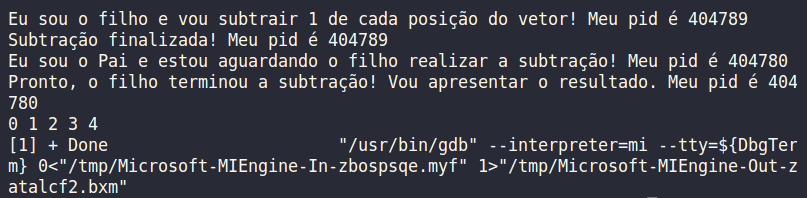
\includegraphics{q2_out}

\subsection*{Explicação}
O programa primeiro printa a seguinte frase : "Eu sou o Pai estou prestes a ter um filho!". Indicando que nesse momento, quem está rodando é o processo pai e o processo filho ainda não existe. Após isso é utilizado o comando fork, onde é criado um novo processo que é o processo filho.\\
    A partir daí, os dois processos, pai e filho, são concorrentes. O output do programa acontece de acordo com as condições explicitadas no código:\\
    Se o processo que está rodando atualmente é o filho, a seguinte frase é printada: "Eu sou o filho e vou subtrair 1 de cada posição do vetor!", a subtração é executada e é printado: Subtração finalizada!".\\
    Caso o processo que está rodando é o pai, temos esse output: "Eu sou o Pai e estou aguardando o filho realizar a subtração!", e então o processo pai espera pelo término do processo filho.\\
    Depois que o processo filho é finalizado, dentro do processo pai a frase "Pronto, o filho terminou a subtração! Vou apresentar o resultado." é printada. E então, o valor do vetor G é apresentado com os valores originais.\\
Note que o vetor G foi criado antes do fork, portanto ele tem o mesmo valor para os dois processos nesse momento.
No caso do processo filho, é feita a subtração. Então o valor de G muda para {-1, 0, 1, 2, 3}. Mas não é apresentado, de acordo com o proposto no enunciado.
Já no processo pai, o valor de G apresentado é o original. Pois não houve a subtração, visto que ela só é feita no processo filho.
